\section{Hyperparameter Exploration}

\subsection{Experiment: Deeper CNN (Option B)}

\textbf{Architecture:} Added a third convolutional layer (64 channels) with MaxPooling to the original CNN.

\begin{itemize}
    \item Validation accuracy: \textbf{99.29\%}
    \item Number of parameters: \textbf{458,570}
    \item Training epochs: \textbf{20}
\end{itemize}

\begin{figure}[h]
    \centering
    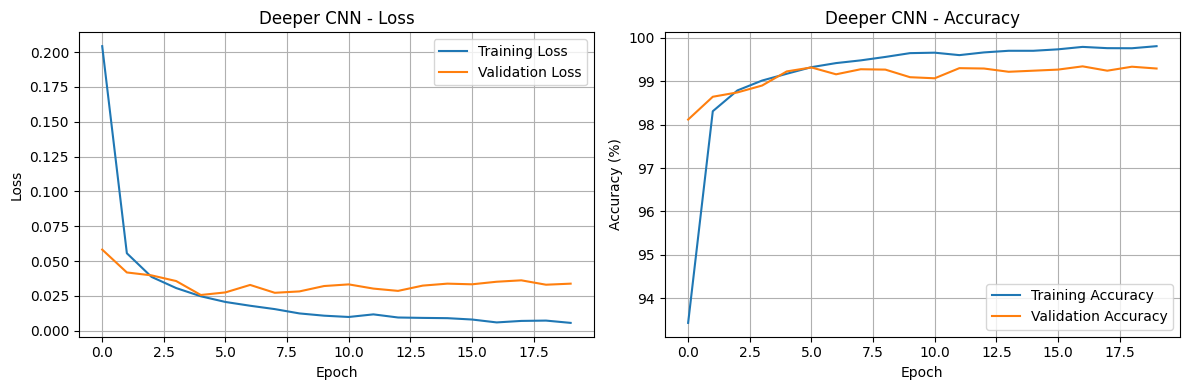
\includegraphics[width=0.7\linewidth]{section4/deeper_cnn.png}
    \caption{Training and validation curves for Deeper CNN}
    \label{fig:deeper-cnn}
\end{figure}

\textbf{Performance Analysis:} The deeper CNN achieved 99.29\% validation accuracy compared to 99.03\% for the original CNN. An improvement of only 0.26\% despite an 8.8\% increase in parameters (36,928 additional). This minimal improvement demonstrates diminishing returns: the 2-layer CNN was already near-optimal for MNIST's complexity.

\subsection{Learning Rate Sensitivity Experiment}

Testing with $\text{learning rate} = 0.1$ (100× larger than optimal 0.001):

\begin{figure}[h]
    \centering
    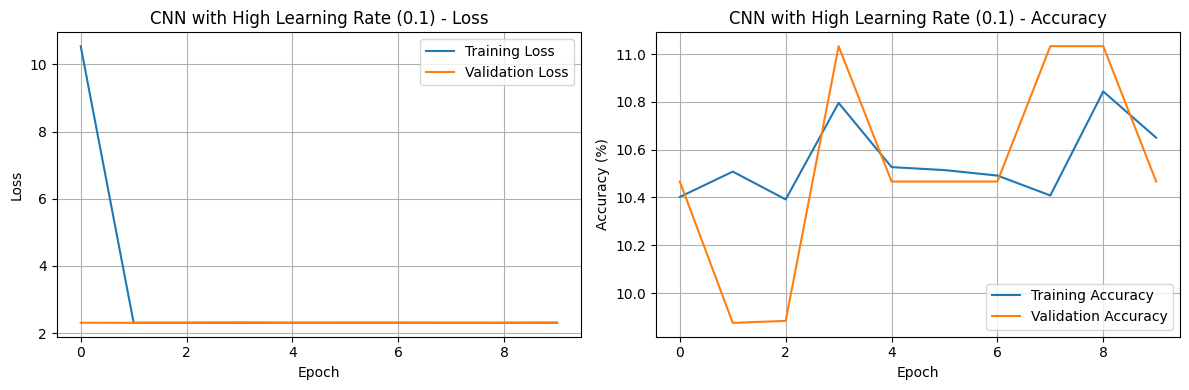
\includegraphics[width=0.7\linewidth]{section4/high_lr.png}
    \caption{Training instability with high learning rate (0.1)}
    \label{fig:high-lr}
\end{figure}

\begin{table}[h]
\centering
\begin{tabular}{|l|c|c|}
\hline
\textbf{Learning Rate} & \textbf{Val Accuracy} & \textbf{Training Loss} \\ \hline
0.001 (normal) & 99.2\% & 0.23 \\ \hline
0.1 (high) & 10.5\% & 10.54 \\ \hline
\end{tabular}
\caption{Impact of excessive learning rate}
\label{tab:lr-comparison}
\end{table}

\subsubsection{Question 4.2: What happened with high learning rate?}

Training with a learning rate of 0.1 completely failed, the model only got 10.5\% accuracy, which is barely better than random guessing (10\% for 10 digits). 

The problem is that the learning rate controls how big of a step the model takes when updating its weights. When I used 0.001, it took small, careful steps and gradually improved. But with 0.1 (which is 100 times bigger), the steps are way too large. Instead of carefully walking down to the bottom of a valley, the model is taking such huge leaps that it keeps overshooting and bouncing around randomly. The training loss just fluctuates wildly between 2.3 and 10.54 with no pattern.

This experiment really showed me that learning rate is probably the most important hyperparameter to get right.